\documentclass[letterpaper, 10pt, DIV=13]{scrartcl}
\usepackage[T1]{fontenc}
\usepackage[english]{babel}
\usepackage{amsmath, amsfonts, amsthm, xfrac}
\usepackage{listings}
\usepackage{color}
\usepackage{longtable}
\usepackage{etaremune}

\numberwithin{equation}{section}
\numberwithin{figure}{section}
\numberwithin{table}{section}

\usepackage{sectsty}
\allsectionsfont{\normalfont\scshape} % Make all section titles in default font and small caps.

\usepackage{fancyhdr} % Custom headers and footers
\pagestyle{fancyplain} % Makes all pages in the document conform to the custom headers and footers

\fancyhead{} % No page header - if you want one, create it in the same way as the footers below
\fancyfoot[L]{} % Empty left footer
\fancyfoot[C]{} % Empty center footer
\fancyfoot[R]{\thepage} % Page numbering for right footer

\renewcommand{\headrulewidth}{0pt} % Remove header underlines
\renewcommand{\footrulewidth}{0pt} % Remove footer underlines
\setlength{\headheight}{13.6pt} % Customize the height of the header

\lstset{numbers=left, numberstyle=\tiny, stepnumber=1, numbersep=5pt}

% Colors and lstset for syntax highlighting from https://www.overleaf.com/latex/examples/syntax-highlighting-in-latex-with-the-listings-package/jxnppmxxvsvk
\definecolor{mygreen}{rgb}{0,0.6,0}
\definecolor{mygray}{rgb}{0.5,0.5,0.5}
\definecolor{mymauve}{rgb}{0.58,0,0.82}

% Define Language
\lstdefinelanguage{rust-eze}
{
  % list of keywords
  morekeywords=[1]{
      import,
      if,
      while,
      for,
      specs,
      model,
      start,
      finish,
      extends,
      ext,
      fn,
      else,
      return
  },
  morekeywords=[2]{
    mut,
    i32,
    u8,
    bool,
    String,
    Vec,
    Tuple,
    true,
    false,
    char,
    self,
    void,
    new
  },
  keywordstyle=[1]\color{blue},
  keywordstyle=[2]\color{red},
  sensitive=true,
  morecomment=[l]{//}, % l is for line comment
  morecomment=[s]{/*}{*/}, % s is for start and end delimiter
  morestring=[b]" % defines that strings are enclosed in double quotes
}

\lstset{
  language={rust-eze},
  backgroundcolor=\color{white},   % choose the background color
  basicstyle=\footnotesize,        % size of fonts used for the code
  breaklines=true,                 % automatic line breaking only at whitespace
  captionpos=b,                    % sets the caption-position to bottom
  commentstyle=\color{mygreen},    % comment style
  escapeinside={\%*}{*},          % if you want to add LaTeX within your code
  stringstyle=\color{mymauve},     % string literal style
}

\setlength\parindent{0pt}
\pagenumbering{gobble}

\title {
	\normalfont
	\huge{Rust-eze} \\
	\vspace{10pt}
	\large{CMPT 331 - Spring 2023 | Dr. Labouseur}
}

\author{\normalfont Josh Seligman | joshua.seligman1@marist.edu}
\date{\normalfont May 10, 2023}

\pagenumbering{arabic}
\begin{document}
\maketitle

\begin{figure}[ht]
  \centering
  
\includegraphics[width = 10cm]{lightning_mcqueen.png}
\end{figure}

\newpage

\section{Introduction}
Rust-eze is modern, object-oriented, type-safe programming language. It inherits
the best parts of Rust and Java to provide a fast and memory-safe languge for
the object-oriented paradim, while also bringing in some syntactic influence from Pascal.
Rust-eze does, however, differ from its parent languages in the following ways:
\begin{enumerate}
    \item Rust-eze is an object-oriented language, which, like Java, means there
          are no structs and only classes/objects.
    \item Like Java, but unlike Rust, Rust-eze requires that all
          variables be explicitly defined with their respective types.
    \item Similar to Rust, but unlike Java, Rust-eze uses a system of borrowing
          and ownership so only one variable can point to a given place in
          memory at a time. This prevents the need for a garbage collector as
          variables are automatically dropped and the memory is freed when they
          go out of scope.
    \item Unlike Java, but like Rust, Rust-eze is compiled into the native
          binary, so there is no need for a JVM or an intermediate bytecode
          representation of Rust-eze programs.
    \item Similar to Rust, all instance variables must be initialized within the
          constructor.
    \item Similar to both parent languages, all models (classes) belong to a garage
          (Java package). However, more similar to Rust, the garage is inferred
          based on the relative file location and does not have to be explicitly
          defined within the file.
\end{enumerate}

\newpage

\subsection{Genealogy}
\begin{figure}[ht]
    \centering
    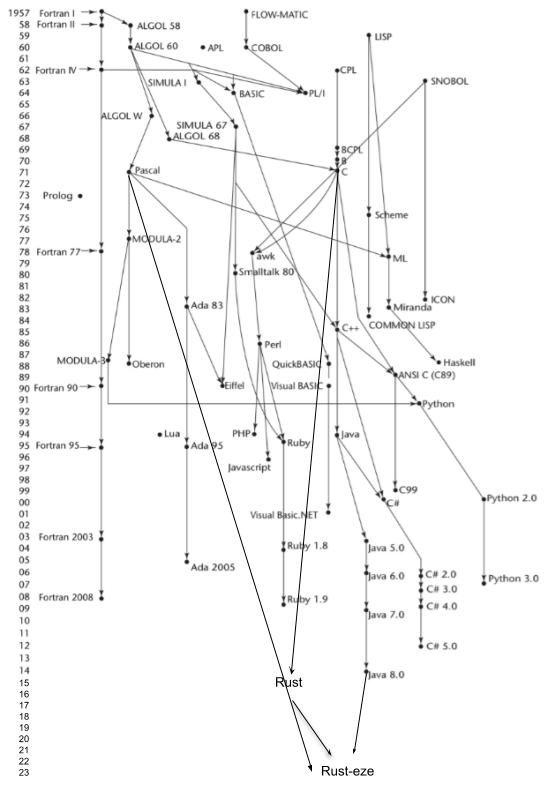
\includegraphics[height=6.5in]{genealogy.jpg}
\end{figure}

\newpage

\subsection{Hello World}
\begin{lstlisting}[caption = HelloWorld.rez, frame = single, nolol]
model HelloWorld
start
    ext fn main(Vec<String> args) -> void
    start
        println("Hello world!");
    finish main
finish model
\end{lstlisting}

\subsection{Program Structure}
The key organizational concepts in Rust-eze are as follows:
\begin{enumerate}
    \item Every file contains a single \textbf{model} (equivalent to a class),
          which should be the same name as the file minus the \textit{.rez} file
          extension.
      \item All instance members default to being in the interior (private) unless they 
          are declared with the \textbf{ext} keyword to note their exterior (public) presence.
    \item Instance variables are declared within the \textbf{specs} block and
          must be initialized within the constructor, which is a function that
          is the same name as the model.
    \item Local variables are immutable by default unless they are declared with
          the \textbf{mut} keyword.
    \item The entry point for all Rust-eze programs is the main method that is
          located in one of the models of the project.
\end{enumerate}

The program below defines a new \textbf{model} called Lightning that contains
3 instance variables: an exterior String called \textit{name}, an exterior
integer called \textit{age}, and an interior integer called \textit{miles}. Each
of these instance variables are initialized within the constructor. Each
Lightning has 2 member functions: \textit{drive} and \textit{say\_it}.
\textit{drive} is an exterior method as it is defined with the \textbf{ext}
keyword. Since it modifies an instance variable, it must take it a mutable
reference to the object in addition to the number of miles being driven. Inside
of the method, a new local variable called \textit{new\_mileage} is declared
without the \textbf{mut} keyword, meaning that it is immutable and is a constant
with the value it is initialized with. The other instance method,
\textit{say\_it}, is also public and does not modify the instance variables,
which is why it needs an immutable reference to \textbf{self}.

\begin{lstlisting}[caption = Lightning.rez, frame = single, nolol]
model Lightning
start
    specs
    start
        ext String name;
        ext i32 age;
        i32 miles;
    finish specs

    ext fn Lightning(String my_name, i32 my_age)
    start
        self.name := my_name;
        self.age := my_age;
        self.miles := 0;
    finish Lightning

    ext fn drive(&mut self, i32 num_miles) -> void
    start
        i32 new_mileage := self.miles + num_miles;
        self.miles := new_mileage;
    finish drive

    ext fn say_it(&self) -> void
    start
        println("Kachow!");
    finish say_it
finish model
\end{lstlisting}

Next, the Lightning model is imported to a new file called \textit{Main.rez}
and is initialized within the main method. Since the \textbf{mut} keyword is
used, we can use the mutable method of \textit{drive} on the new object as well
as directly modify its exterior specs. After \textit{the\_lightning}'s
name is printed, we call its \textit{say\_it} method and then call the
\textit{drive} method with an input of 42 miles to increase the object's mileage.

\begin{lstlisting}[caption = Main.rez, frame = single, nolol]
import garage.Lightning;

model Main
start
    ext fn main(Vec<String> args) -> void
    start
        mut Lightning the_lightning := new Lightning("McQueen", 17);
        println(the_lightning.name);

        the_lightning.say_it();
        the_lightning.drive(42);
    finish main
finish model
\end{lstlisting}

\subsection{Types and Variables}
There are two kinds of variables in Rust-eze: \textbf{\textit{value types}} and
\textbf{\textit{reference types}}. Variables of value types directly contain
their data, while variables of reference types store references to their data or
objects in memory. Due to the ownership system, only one variable of a reference
type can point to a particular place in memory at a given time. See Section 3
for details.

\subsection{Visibility}
In Rust-eze, visibility of methods and instance variables is defined as either
interior (private) or exterior (public). Everything is part of the interior unless
explicitly stated to be in the exterior. Once a variable or method is public,
it may be accessed outside of the model in which it is defined.

\subsection{Statements Differing from Rust and Java}
\begin{center}
\begin{longtable}{|p{2in}|p{4in}|}
\hline
\textbf{Statement} & \textbf{Example} \\
\hline
Assignment statement & \begin{lstlisting}[nolol, numbers = none]
mut i32 x := 5;
x := 3;
i32 y := x + 2;
\end{lstlisting} \\
\hline
If statement & \begin{lstlisting}[nolol, numbers = none]
i32 x := 7;
if x > 3 && x < 9
start
    println("Hello there");
else
    println("Kachow");
finish if
\end{lstlisting} \\
\hline
For loop & \begin{lstlisting}[nolol, numbers = none]
for mut i32 i in range(0, 10, 1)
start
    println(i);
finish for
\end{lstlisting} \\
\hline
While loop & \begin{lstlisting}[nolol, numbers = none]
mut i32 i := 0;
while i < 10
start
    println(i);
    i := i + 1;
finish while
\end{lstlisting} \\
\hline
\end{longtable}
\end{center}

\section{Lexical Structure}
\subsection{Programs}
A Rust-eze program consists of one or more source files. A source file is an
ordered sequence of (probably) Unicode characters. 
\\ \\
Conceptually speaking, a program is compiled using five steps:
\begin{enumerate}
    \item Transformation, which converts a file from a particular character
          repertoire and encoding scheme into a sequence of Unicode characters.
    \item Lexical analysis, which translates a stream of Unicode input
          characters into a stream of tokens.
    \item Syntactic analysis (parsing), which translates the stream of tokens
          into a concrete syntax tree (CST).
    \item Semantic analysis, which converts the CST into an abstract syntax tree
          (AST) and is passed to the semantic analyzer for scope and type
          checking and the borrow checker to make sure all variables
          referenced are active owners of data.
    \item Code generation, which converts the AST into executable code for the
          target platform and CPU architecture.
\end{enumerate}
\subsection{Grammars}
This specification presents the syntax of the Rust-eze programming language
where it differs from Rust and Java.
\subsubsection{Lexical grammar (tokens) where different from Rust and Java}
<assignment operator> $\rightarrow$ := \\
<block begin> $\rightarrow$ start \\
<block end> $\rightarrow$ finish \\
<print> $\rightarrow$ println \\
<visibility modifier> $\rightarrow$ ext | $\epsilon$ \\
<mutability modifier> $\rightarrow$ mut | $\epsilon$ \\

\subsubsection{Syntactic ("parse") grammar where different from Rust and Java}
<model definition> $\rightarrow$ model <model name> <parent declaration> 
                                 <block begin> <statements> \\
                                 \hspace*{3.5cm}<block end> model \\
<parent declaration> $\rightarrow$ extends <parent model name> | $\epsilon$ \\
<specs definition> $\rightarrow$ specs <block begin> <spec definition> <block end> specs \\
<spec definition> $\rightarrow$ <visibility modifier> <type> <spec name>;
                                <spec definition> | $\epsilon$ \\
<variable declaration> $\rightarrow$ <mutability modifier> <type> <variable name>
                                     <assignment operator>\\
                                     \hspace*{4.2cm}<expression>; \\
<if statement> $\rightarrow$ if <condition> <block begin> <statements> else <statements> <block end> if \\
<for loop> $\rightarrow$ for mut <type> <var name> in <expr> <block begin>
                         <statements> <block end> for \\
<while loop> $\rightarrow$ while <condition> <block begin> <statements> <block end> while \\
<function definition> $\rightarrow$ <visibility modifier> fn <function name>
                                    (<parameter list>) -> <return type> \\
                                    \hspace*{4cm}<block begin> <statements> <block end> <function name>\\
<parameter list> $\rightarrow$ <type> <parameter name>, <parameter list> | $\epsilon$

\subsection{Lexical Analysis}
\subsubsection{Comments}
Rust-eze supports two forms of comments: single-line and multi-line comments.
Single-line comments start with the characters // and extend to the end of the
line in the source file. Multi-line comments begin with /* and end with */ and
may span multiple lines. Comments do not nest.

\subsection{Tokens}
There are several kinds of tokens: identifiers, keywords, literals, operators, 
and punctuators. White space and comments are not tokens, though they act as
separators for tokens where needed. \\
Tokens:
\begin{itemize}
    \item identifier
    \item keyword
    \item integer literal
    \item real literal
    \item character literal
    \item string literal
    \item operator or punctuator
\end{itemize}

\subsubsection{Keywords Different from Rust and Java}
\textbf{New keywords:} range, model, specs, start, finish, ext, Tuple \\
\textbf{Removed keywords:} use, class, match, do, private, byte, short, str,
                           boolean, static, public, double, long, float,
                           int, as, pub, impl, struct \\

\section{Type System}
Rust-eze uses a strong static type system. This means that the Rust-eze compiler
will catch type mismatch errors at compile time through early binding compile-time
type checking.

\subsection{Type Rules}
The type rules for Rust-eze are as follows: \\ \\
S $\vdash$ e1 : T \\
S $\vdash$ e2 : T \\
T is a primitive type \\
--------------------------- \\
S $\vdash$ e1 := e2 : T \\
\\
S $\vdash$ e1 : T \\
S $\vdash$ e2 : T \\
T is a primitive type \\
--------------------------- \\
S $\vdash$ e1 == e2 : bool \\
\\
S $\vdash$ e1 : T \\
S $\vdash$ e2 : T \\
T is a primitive type \\
--------------------------- \\
S $\vdash$ e1 != e2 : bool \\
\\
S $\vdash$ e1 : T \\
S $\vdash$ e2 : T \\
T is a numeric primitive type \\
--------------------------------------- \\
S $\vdash$ e1 > e2 : bool \\
\\
S $\vdash$ e1 : T \\
S $\vdash$ e2 : T \\
T is a numeric primitive type \\
--------------------------------------- \\
S $\vdash$ e1 < e2 : bool \\
\\
S $\vdash$ e1 : T \\
S $\vdash$ e2 : T \\
T is a numeric primitive type \\
--------------------------------------- \\
S $\vdash$ e1 + e2 : T \\
\\
S $\vdash$ e1 : String \\
S $\vdash$ e2 : T with a String representation \\
--------------------------------------------------- \\
S $\vdash$ e1 + e2 : String


\subsection{Value Types}
\begin{center}
\begin{longtable}{|p{3in}|p{3in}|}
    \hline
    \textbf{Data Type} & \textbf{Description} \\
    \hline
    i8, i16, i32, i64 & Signed integers that store up to X bits, where X is the
                        number after "i" in the data type. \\
    \hline
    u8, u16, u32, u64 & Unsigned integers that store up to X bits, where X is the
                        number after "u" in the data type. \\
    \hline
    f32, f64 & Floating point numbers that store up to X bits, where X is the
               number after "f" in the data type. \\
    \hline
    bool & Boolean value that can be either \textbf{false} or \textbf{true}. \\
    \hline
    char & Character value that stores the data for a single character. \\
    \hline
\end{longtable}
\end{center}

\subsection{Reference Types}
\begin{center}
\begin{longtable}{|p{3in}|p{3in}|}
    \hline
    \textbf{Data Type} & \textbf{Description} \\
    \hline
    String & A sequence of characters. \\
    & Example: \begin{lstlisting}[nolol, numbers = none]
    String x := "hello";
    \end{lstlisting} \\
    \hline
    Vec<T> & A dynamic, homogeneous array of values of type T, which can be any type. \\
    & Example: \begin{lstlisting}[nolol, numbers = none]
    Vec<i32> nums1 := [0, 0, 7];
    mut Vec<i32> nums2 := new Vec<i32>(2);
    nums2[0] := 42;
    nums2[1] := 99;
    \end{lstlisting} \\
    \hline
    Tuple & A collection of values of different types that is fixed in size. \\
    & Example: \begin{lstlisting}[nolol, numbers = none]
    Tuple<i32, bool, i32> my_tuple := (7, false, 3);
    mut Tuple<String, i32> the_tuple := new Tuple<String, i32>();
    the_tuple.0 := "jOSh";
    the_tuple.1 := 2;
    \end{lstlisting} \\
    \hline
\end{longtable}
\end{center}

\section{Example Programs}
\subsection{Caesar Cipher Encrypt}
\begin{lstlisting}[caption = CaesarCipher.rez, frame = single, nolol]
// Model definition for the Caesar cipher
model CaesarCipher
start
    // Encryt a string based on the shift amount
    ext fn encrypt(&self, &String in_str, i32 shift_amt) -> String
    start
        // Get the real shift amount and create a new vector of characters
        i32 real_shift := shift_amt % 26;
        Vec<char> out_vec := new Vec<char>();

        // Loop through the entire string
        for mut i32 i in range(0, in_str.len(), 1)
        start
            
            // Get the character at the given index as an integer
            // (u8) casts the expression on the right of it to be an u8
            mut u8 cur_char := (u8) in_str.char_at(i);

            if cur_char >= 97 && cur_char <= 122
            start
                // Convert the lowercase letters to uppercase letters
                cur_char := cur_char - 32;
            finish if

            // Only modify uppercase letters
            if cur_char >= 65 && cur_char <= 90
            start
                // Perform the shift
                cur_char := cur_char + real_shift;

                // This is the difference for wraparound for Z
                mut i32 diff := cur_char - 90;
                if diff > 0
                start
                    // Perform the Z wraparound
                    cur_char := 65 + diff - 1;
                else
                    // Now compute the A wraparound if there was no Z wraparound
                    diff := 65 - cur_char;

                    if diff > 0
                    start
                        cur_char := 90 - diff + 1;
                    finish if
                finish if
            finish if
            
            // Get the final character as the appropriate type
            char final_char := (char) cur_char;

            // Push it to the end of the vector (vector will resize as needed)
            out_vec.push(final_char);
        finish for

        // Join the elements of the vector together to form a string
        // by using the string representation of each of the elements
        return out_vec.join("");
    finish encrypt

    ext fn main(Vec<String> args) -> void
    start
        CaesarCipher cipher := new CaesarCipher();

        // Create a new string
        String x := "Kachow";
        
        // Perform encrypt and pass an immutable reference to x
        String y := cipher.encrypt(&x, 95);

        // Should print Kachow
        println(x);
        // Should print BRTYFN
        println(y);
    finish main
finish model
\end{lstlisting}
\subsection{Caesar Cipher Decrypt}
\begin{lstlisting}[caption = CaesarCipher.rez (enhanced), frame = single, nolol]
model CaesarCipher
start
    // Returns a decrypted string based on the shift amount
    ext fn decrypt(&self, &String in_str, i32 shift_amt) -> String
    start
        // Decrypt is the same as encrypt with negative shift amount
        // Encrypt is defined in Section 4.1
        return self.encrypt(in_str, -shift_amt);
    finish encrypt

    ext fn main(Vec<String> args) -> void
    start
        CaesarCipher cipher := new CaesarCipher();

        String x := "Kachow";
        String y := cipher.encrypt(&x, 95);
        String z := cipher.decrypt(&y, 95);
        // Kachow
        println(x);
        // BRTYFN
        println(y);
        // KACHOW
        println(z);
    finish main
finish model
\end{lstlisting}

\subsection{Factorial}
\begin{lstlisting}[caption = FatorialProgram.rez, frame = single, nolol]
// Define a model for the factorial program
model FactorialProgram
start
    // Return the result of factorial(num)
    ext fn factorial(&self, i32 num) -> i32
    start
        if num <= 0
        start
            // factorial(0) = 1
            // and anything < 0 is invalid, so return 1
            return 1;
        else
            // factorial(n) = n * factorial(n - 1)
            return num * self.factorial(num - 1);
        finish if
    finish factorial

    ext fn main(Vec<String> args) -> void
    start
        FactorialProgram fp := new FactorialProgram();
        // Should be 120
        println(fp.factorial(5));

        // Both should be 1
        println(fp.factorial(0));
        println(fp.factorial(-1));
    finish main
finish model
\end{lstlisting}

\subsection{Quicksort}
\begin{lstlisting}[caption = SortsAndShuffles.rez, frame = single, nolol]
// Import the Random model for use later
import std.util.Random;

// Define a model for the classic SortsAndShuffles file from algorithms
model SortsAndShuffles
start
    // This is the wrapper function for the quicksort implementation
    ext fn quicksort(&self, &mut Vec<i32> data) -> void
    start
        // Call quicksort on the entire vector
        self.quicksort_with_indices(data, 0, data.len() - 1);
    finish quicksort

    // Helper quicksort function
    // Private because only accessible within the model
    fn quicksort_with_indices(&self, &mut Vec<i32> data, i32 start_index, i32 end_index) -> void
    start
        // Recursion base case to end if we have an array of size 0 or 1
        if start_index >= end_index
        start
            return;
        finish if

        // Declare a pivot index that will be changed in a few lines
        mut i32 pivot_index := 0;

        if end_index - start_index < 3
        start
            // Pivot index is the start index because will need one more level
            // of recursion regardless of the pivot
            pivot_index := start_index;
        else
            // Otherwise declare a new random object
            Random ran := new Random();

            // Get the first pivot option
            i32 pivot_choice_1 := ran.randInt(start_index, end_index + 1);

            // Get the second pivot option, but only use it if different from
            // the first
            mut i32 pivot_choice_2 := ran.randInt(start_index, end_index + 1);
            while pivot_choice_2 == pivot_choice_1
            start
                pivot_choice_2 := ran.randInt(start_index, end_index + 1);
            finish while

            // Get the third pivot option but only use it if different from
            // both of the other options
            mut pivot_choice_3 := ran.randInt(start_index, end_index + 1);
            while pivot_choice_3 == pivot_choice_1 || pivot_choice_3 == pivot_choice_2
            start
                pivot_choice_3 := ran.randInt(start_index, end_index + 1);
            finish while

            // Get the median of the pivots and set the appropriate pivot index
            if data[pivot_choice_1] <= data[pivot_choice_2] && data[pivot_choice_1] >= data[pivot_choice_3]
            start
                pivot_index := pivot_choice_1;
            else if data[pivot_choice_1] <= data[pivot_choice_3] && data[pivot_choice_1] >= data[pivot_choice_2]
                pivot_index := pivot_choice_1;
            else if data[pivot_choice_2] <= data[pivot_choice_1] && data[pivot_choice_2] >= data[pivot_choice_3]
                pivot_index := pivot_choice_2;
            else if data[pivot_choice_2] <= data[pivot_choice_3] && data[pivot_choice_2] >= data[pivot_choice_1]
                pivot_index := pivot_choice_2;
            else
                pivot_index := pivot_choice_3;
            finish if
        finish if
        
        // Perform the partition
        i32 partition_out := self.partition(data, start_index, end_index, pivot_index);

        // Perform quicksort on the 2 sides of the partition
        self.quicksort_with_indices(data, start_index, partition_out - 1);
        self.quicksort_with_indices(data, partition_out + 1, end_index);

    finish quicksort_with_indices

    // Delare a private function for sorting the array that returns the index
    // for the partition
    fn partition(&self, &mut Vec<i32> data, i32 start_index, i32 end_index, i32 pivot_index) -> i32
    start
        // Move the pivot to the end of the array
        i32 pivot := data[pivot_index];
        data[pivot_index] := data[end];
        data[end] := pivot;

        // Keep track of where the low partition starts
        mut i32 last_low_partition_index := start_index - 1;

        // Go through the sub array, excluding the last index because the pivot
        // value is in the end index
        for mut i in range(start_index, end_index, 1)
        start
            if data[i] < pivot
            start
                // Make space for the low value
                last_low_partition_index := last_low_partition_index + 1;

                // Move it to its new spot in the array
                i32 temp := data[i];
                data[i] := data[last_low_partition_index];
                data[last_low_partition_index] := temp;
            finish if
        finish for

        // Move the pivot to the appropriate location
        data[end] := data[last_low_partition_index + 1];
        data[last_low_partiton_index + 1] := pivot;

        // Return the location of the pivot to distinguish the 2 partitions
        return last_low_partition_index + 1;
    finish partition

    // Knuth shuffle
    ext fn knuth_shuffle(&self, &mut Vec<i32> data) -> void
    start
        // Create the random object
        Random ran := new Random();

        // Iterate through the entire array
        for mut i32 i in range(0, data.len(), 1)
        start
            // Get a random index
            i32 swap_index := ran.randInt(0, data.len()));

            // Swap the 2 elements
            i32 temp := data[i];
            data[i] := data[swap_index];
            data[swap_index] := temp;
        finish for

    finish knuth_shuffle

    ext fn main(Vec<String> args) -> void
    start
        // Initialize a vector with initial capacity for 10 elements
        mut Vec<i32> my_arr := new Vec<i32>(10);
        // Fill the vector with values 0 - 9
        for mut i32 i in range(0, 10, 1)
        start
            my_arr[i] := i;
        finish for
        
        SortsAndShuffles sas := new SortsAndShuffles();

        // Shuffly the vector
        sas.knuth_shuffle(&mut my_arr);
        println(my_arr.to_string());

        // Sort the vector
        sas.quicksort(&mut my_arr);
        println(my_arr.to_string());
    finish main

finish model
\end{lstlisting}

\subsection{Selection Sort}
\begin{lstlisting}[caption = SortsAndShuffles.rez (enhanced), frame = single, nolol]
// Import random for the Knuth shuffle defined in Section 4.4
import std.util.Random;

model SortsAndShuffles
start
    // Create a public function for doing a selection sort
    ext fn selection_sort(&self, &mut Vec<i32> data) -> void
        // Loop through all but the last element because an array of length 1
        // is already sorted
        for mut i32 i in range(0, data.len() - 1, 1)
        start
            // Assume first element is smallest
            // Can directly assign here because i32 is a value type, so the value
            // gets stored rather than the actual reference
            mut i32 smallest_index := i;
            
            // Go through the rest of the array
            for mut i32 j in range(i + 1, data.len(), 1)
            start
                // If we have a smaller element, save the new lower index
                if data[smallest_index] > data[j]
                start
                    smallest_index := j;
                finish if
            finish for

            // Move the smallest element in place
            i32 temp := data[i];
            data[i] := data[smallest_index];
            data[smallest_index] := temp;
        finish for
    finish selection_sort

    ext fn main(Vec<String> args) -> void
    start
        // From Section 4.4
        mut Vec<i32> my_arr := new Vec<i32>(10);
        for mut i32 i in range(0, 10, 1)
        start
            my_arr[i] := i;
        finish for
        
        SortsAndShuffles sas := new SortsAndShuffles();

        // Shuffle (from Section 4.4)
        sas.knuth_shuffle(&mut my_arr);
        println(my_arr.to_string());

        // Sort
        sas.selection_sort(&mut my_arr);
        println(my_arr.to_string());
    finish main
finish model
\end{lstlisting}

\subsection{Object-Oriented Programming With Transformers}
\begin{lstlisting}[caption = Owner.rez, frame = single, nolol]
model Owner
start
    specs
    start
        // Every owner has a name
        ext String name;
    finish specs

    // Define a new owner with the given name
    ext fn Owner(String my_name)
    start
        self.name := my_name;
    finish Owner
finish model
\end{lstlisting}

\begin{lstlisting}[caption = Transformer.rez, frame = single, nolol]
import garage.Owner;

model Transformer
start
    specs
    start
        ext String name;
        ext String car_name;
        i32 power;
        &Transformer leader;
        &Owner owner;
    finish specs

    // Define a constructor for the Transformer
    ext fn Transformer(String my_name, String my_car_name, i32 power)
    start
        self.name := my_name;
        self.car_name := my_car_name;
        self.power := power;

        // Leader and owner have to be set by setters, so null at first
        // Also follow the rule that all specs are initialized in the constructor
        self.leader := null;
        self.owner := null;
    finish Transformer

    // Returns the difference in power when attacking another transformer
    // > 0 means win
    // < 0 means loss
    // == 0 means draw
    ext fn attack(&self, &Transformer oponent) -> i32
    start
        mut i32 power_diff := self.power - oppenent.get_power();
        
        &Transformer oppenent_leader := oppenent.get_leader();
        if oppenent_leader != null
        start
            // We will say the leader helps out if their comrade is being attacked
            power_diff := power_diff - oppenent_leader.get_power();
        finish if

        return power_diff;
    finish attack

    // Increases the power of the transformer by the factor
    ext fn supercharge(&mut self, i32 factor)
    start
        self.power := self.power * factor;
    finish supercharge

    // Define a getter for the power spec
    ext fn get_power(&self) -> i32
    start
        return self.power;
    finish get_power

    // Define a getter for the leader spec
    ext fn get_leader(&self) -> &Transformer
    start
        return self.leader;
    finish get_leader

    // Define a setter for the leader
    ext fn set_leader(&mut self, &Transformer new_leader)
    start
        self.leader := new_leader;
    finish set_leader

    // Define a setter for the owner
    ext fn set_owner(&mut self, &Owner new_owner)
    start
        self.owner := new_owner;
    finish set_owner
finish model
\end{lstlisting}

\begin{lstlisting}[caption = Autobot.rez, frame = single, nolol]
import garage.Transformer;

// Autobot is a subclass/model of Transformer
model Autobot extends Transformer
start
    ext fn Autobot(String my_name, String my_car_name, i32 power)
    start
        // All specs are initialized in the super constructor, so nothing
        // needs to be explicitly initialized here
        super(my_name, my_car_name, power);
    finish Autobot

    // Function to "roll out"
    ext fn roll_out(&self)
    start
        println("Roll out: " + self.name);
    finish roll_out
finish model
\end{lstlisting}

\begin{lstlisting}[caption = MainTransformers.rez, frame = single, nolol]
import garage.Owner;
import garage.Transformer;
import garage.Autobot;

model MainTransformers
start
    ext fn main(Vec<String> args) -> void
    start
        // Create a new autobot for Bumblebee
        mut Autobot bumblebee := new Autobot("Bumblebee", "Chevy Camaro", 500);

        // Give Bumblebee an owner
        Owner sam := new Owner("Sam Witwicky");
        // This method is accessible because Autobot extends Transformer
        bumblebee.set_owner(&sam);

        Autobot optimus_prime := new Autobot("Optimus Prime", "Truck", 1000);
        // Give a reference to Optimus Prime for Bumblebee's leader
        bumblebee.set_leader(&optimus_prime);

        // Create Megatron
        Transformer megatron := new Transformer("Megatron", "Tank", 2000);
        
        // This will be 500 because Bumblebee gets assistance from Optimus Prime
        // but their combined power is too low
        println(megatron.attack(&bumblebee));
        
        // Should be -1000 because the difference in their power is 1000 and
        // Megatron has no leader
        println(optimus_prime.attack(&megatron));

        // Multiply Bumblebee's power by a factor of 3
        bumblebee.supercharge(3);

        // This will be -500 because Bumblebee is now at 1500 power
        // plus Optimus Prime's 1000 power
        println(megatron.attack(&bumblebee));

        // Optimus Prime has the function because he is an Autobot
        // Megatron does not because it is only defined in the Autobot model
        optimus_prime.roll_out();
    finish main
finish model
\end{lstlisting}
\end{document}
